\documentclass[12pt]{article}
\usepackage{geometry}
\usepackage{graphicx} % 插图
\usepackage{float} % 插图位置固定
\usepackage{amsmath} % 文字加粗
\usepackage[UTF8]{ctex} %中文宏包
\setCJKmainfont{SimSun}
\usepackage{fontspec} %引入字体设置宏包
\setmainfont{Times New Roman}
\usepackage{indentfirst} %首行缩进
\usepackage{listings} %代码
\usepackage{color} %字体颜色
\usepackage{subfigure}  %插入多图时用子图显示的宏包

\usepackage{minted} %代码
\usemintedstyle{vs}


%\usepackage{fancyhdr} %页眉页脚
%\pagestyle{fancy} 
%\fancyhf{}
%\lhead{数字图像处理}
%\chead{Noise Reduction Using a Median Filter}
%\rhead{张青铭 \quad 3200105426}
%\renewcommand{\headrulewidth}{0pt}
%图片路径
\graphicspath{ {figures/} }

%页面格式
\geometry{a4paper,
	left=20mm,
	right=20mm,
	top=20mm,
	bottom=20mm }

\title{{\Huge{\textbf{数字图像处理}}}\\Pro5-2\quad  Noise Reduction Using a Median Filter}
\author{信息与电子工程学院\quad 信息工程 \quad 3200105426\\张青铭}
\date{\today}

\begin{document}
	\maketitle
	\section{实验任务}
	(1)设计3*3中值滤波器;
	
	(2)下载图5.7(a),添加椒盐噪声Pa=Pb=0.2;
	
	(3)利用设计的中值滤波器进行滤波,解释滤波前后和图5.10(b)的差异;
	\section{算法设计}
	中值滤波器的设计公式为 $ \hat{f}(x,y)=median_{(s,t)\in S_{xy}}{g(s,t)} $,即选取一个3*3的矩阵作为邻域后,选取其中的中值作为目标图像的像素结果。图像的空域卷积处理为了边界不超出范围需要对原图像进行扩展,因为所用空间滤波器大小为3*3,故扩展行数与列数为原行数列数加2。matlab中首先建立扩展后的全零矩阵,在利用padarray将原始图像赋值给扩展矩阵。空间滤波可以对图像每一个像素点进行遍历,在利用median函数进行选取中值。添加椒盐噪声利用imnoise函数完成。
	\section{代码实现}
	\begin{minted}[frame=lines,tabsize=4,python3,baselinestretch=0.85]{matlab}
clear; clc; close all
%% 主函数
image= imread('./5_7.TIF');

% 原图像
subplot(1, 3, 1)
imshow(image)
title('original image')

% 加噪图像
image_noise = iamnoise(image, 'salt & pepper', 0.2);
subplot(1, 3, 2)
imshow(image_noise)
title('image with salt & papper noise')

% 恢复图像
image_filtered = median_filter(image_noise);
subplot(1, 3, 3)
imshow(image_filtered)
title('image after median filter')
%% 3*3中值滤波器
function image_filter = median_filter(image) % 彩色图中值滤波器

% 获取图像大小
[rows, cols, k] = size(image);

% 创建矩阵,用于存储结果
image_filter = zeros(rows, cols, 'uint8');

% 对边界像素进行扩展
image_extend = zeros(rows+2, cols+2, 'uint8');
image_extend(:,:) = padarray(image(:,:), [1, 1]);

for i = 1:rows
	for j = 1:cols
		Rect = double(image_extend(i:i+2, j:j+2));
		image_filter(i, j) = uint8(median(Rect, 'all')); 
	end
end

end
	\end{minted}
	\section{实验结果}
	对于图像5.7(a),设置椒盐噪声参数0.2,运行上述代码得到结果如下。
	
	原图、加入椒盐噪声以后以及中值滤波后的结果如图所示,总体上可以完成对椒盐噪声的滤除,图像也能恢复为原始情况,只有少量噪点存在。
	\begin{figure}[H]
		\centering
		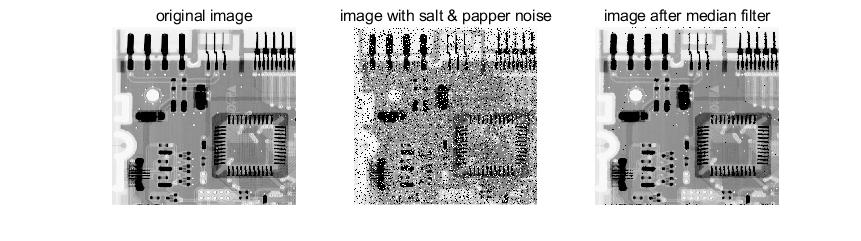
\includegraphics[width=0.9\linewidth]{figures/r1}
		\caption{中值滤波}
	\end{figure}
	
	图2展示了自行设计的中值滤波与标准的中值滤波后的结果,可以发现几乎没有差别,设计思路与设计结果都比较理想。
	\begin{figure}[H]
		\centering
		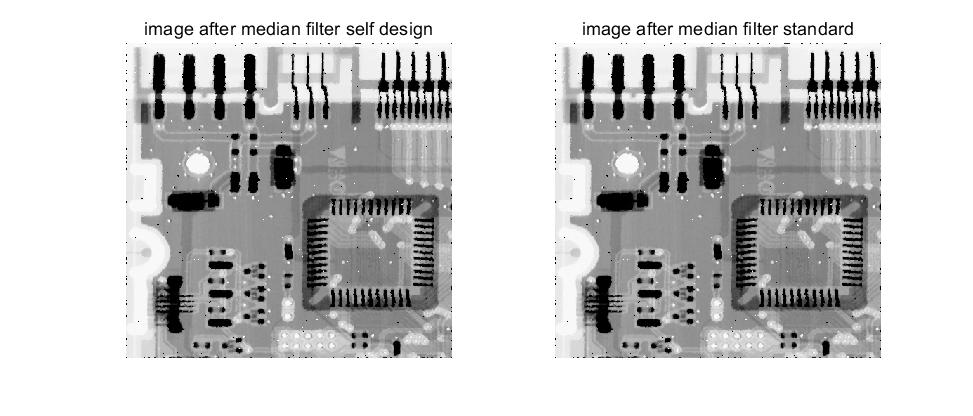
\includegraphics[width=0.7\linewidth]{figures/r2}
		\caption{与标准中值滤波对比}
	\end{figure}
	\section{总结}
	本次实验的核心在于空间滤波器的设计。对于3*3的空间滤波可以用遍历加取中值实现。需要注意的地方有最好能够先定义滤波后的图像矩阵,可以加快代码的运行速度;需要对原图进行范围扩展,以防止超出原图的边界范围。这次实验总体难度不大,对于理解图像的空域处理和卷积操作有很大帮助。
\end{document}
